\subsection{5-1 Queue}

\subsubsection*{Experiment}

\paragraph{By varying the delay times demonstrate that the system works in the manner expected.}


Producer delay: 500

Consumer delay: 0

\begin{tabular}{c|c|c}
	\hline

	Producer delay &
	Consumer delay &
	Results \\
	\hline

	500 &
	0 &
	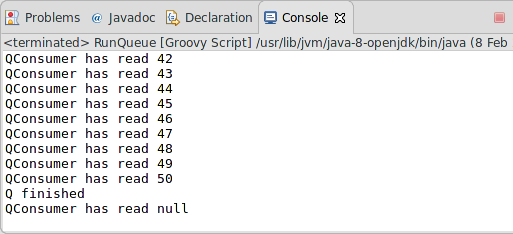
\includegraphics[width=\textwidth / 2]{img/screenshots/5-1-1.png} \\
	\hline

	0 &
	500 &
	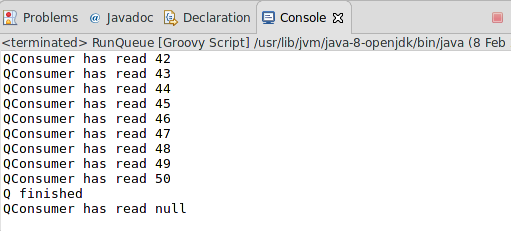
\includegraphics[width=\textwidth / 2]{img/screenshots/5-1-2.png} \\
	\hline

	500 &
	500 &
	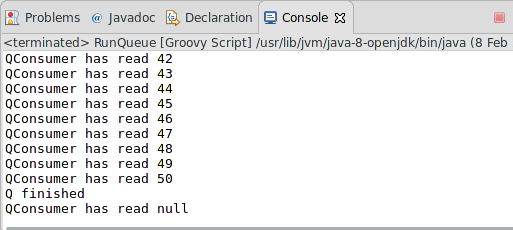
\includegraphics[width=\textwidth / 2]{img/screenshots/5-1-3.png} \\
	\hline

\end{tabular}

\subsubsection*{Questions}

\paragraph{What do you conclude from these experiments?}

From these results we can conclude that the queue class successfully stores and retrieves values as any queue should.  We can also conclude that if a process attempts to read a value from an empty queue, the read will block until a value is inserted into the queue.  The opposite is also true, if a process attempts to write a value into a full queue, the write will block until a value is popped from the queue.
